\chapter{Protocols and Related Works}
\label{chap: Related works}

\textit{This chapter describes the attempts on Cryptography protocols behind the existing HD wallets as 
well as the attempt of adapting these mechanisms to curve ed25519. We analyze the famous wallet that the community are using.}

\minitoc

\section{Protocol proposals}
\subsection{Key derivation}

The word “Hierarchical Deterministic” in crypto wallet were first introduced by Pieter Wuille in Bitcoin Improvement Proposal number 32 (BIP32)\cite{github/bip0032}. The initial idea was to build a wallet architect like a tree. From the root seed, we can derive child private keys and child public keys that construct many child wallets for different purposes. However, BIP32 only supports the elliptic curve used in Bitcoin, defined by the name "secp256k1" \cite{secp256k1}. SatoshiLabs Improvement Proposal number 10 (SLIP10) is an attempt to generalize the BIP32's key derivation schema for different curves, e.g., NIST P-256 and ed25519. For some security reasons, SLIP10 forbade normal child key derivation on curve ed25519. But SLIP23 adopted them both and proposed a new schema on curve Edwards25519 called "BIP32-ed25519" \cite{Khovratovich2017}. In this section, we will explain how these schemes work and analyze the difficulties in adapting BIP32 to the Edwards25519 Curve.

\subsubsection{BIP32}

The most significant motivation of BIP32 is how one can calculate the public key of another without revealing the private keys or the sender has to generate it from private keys. Elliptic curve mathematics permits these kinds of schemes. For example, a webshop business lets its web server generate fresh addresses (public key hashes) for each order or for each customer, without giving the webserver access to the corresponding private keys (which are required for spending the received funds). 

BIP32 also makes wallets more recoverable since users only have to maintain the root seed and a list of wallet indexes. In the example of a webshop, the web owner doesn’t have to keep all the private keys safe, and this becomes more redundant if the owner has an increase in a business requiring more wallets. Instead, he only has to create the seed one and save the indexes each time he makes a wallet. The next part will cover the indexes of children’ wallets and how we can recover the entire wallet structure using the initial seed and list of indexes. 

\bigskip
{\textbf{Derivation}}

BIP 32 key derivation is a mechanism used to generate a specific ECDSA key pair within a tree of indexes. Given a parent extended key and an array of indexes, we will be able to deterministically regenerate keys at that specified index in the tree. Starting from a master seed to the creation of one master extended key, we can create a tree with infinite depth. Each node can also have a maximum of 4,294,967,296 child nodes (2³²/32-bit unsigned integer) resulting in an incredible ability to generate a limitless number of keys. \autoref{fig:bip32} is an example of a BIP32 key tree with depth 3.

\begin{figure}[ht!]
  \centering
  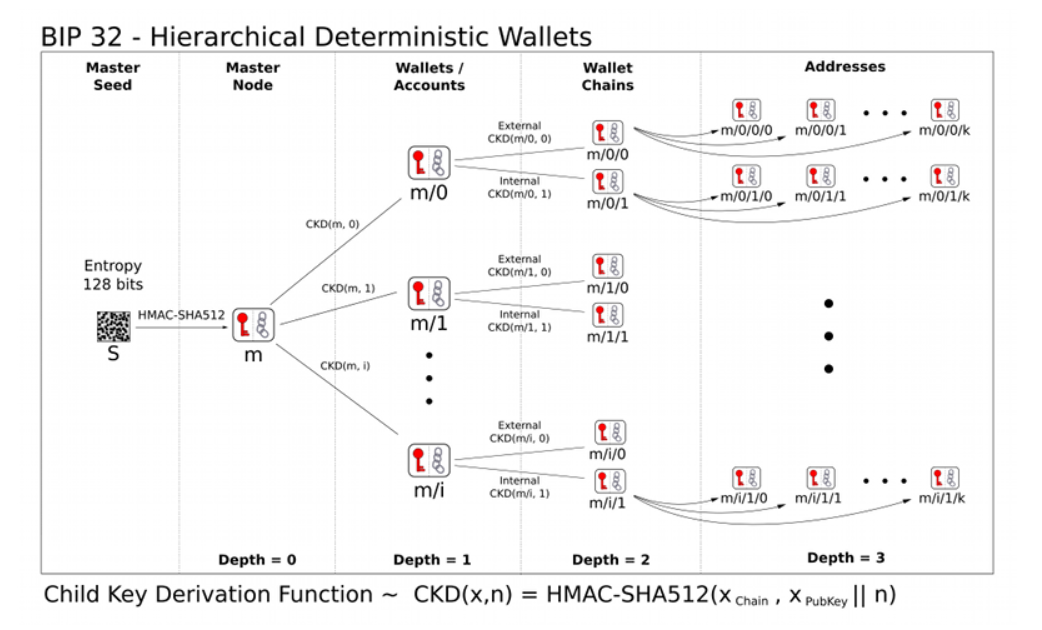
\includegraphics[width=1\textwidth]{images/bip32.png}
  \caption[Example of BIP32 key tree with depth 3]{Example of BIP32 key tree with depth 3}
  \label{fig:bip32}
\end{figure}


\bigskip
{\textbf{Extended keys}}

An extended key is defined as follow: 

\begin{adjustwidth}{2cm}{}
    An extended key consists of a private or public key and chain code. An extended key can create children, generating its own branch in the tree structure. Sharing an extended key gives access to the entire branch.
\end{adjustwidth}

The term "extended key" could also be thought of as "extensible key" because such a key can be used to derive children. BIP32 extends both private and public keys first with an extra chain code. This extension is added in order to prevent depending solely on the key itself; it also is identical for corresponding private and public keys.

In total, an extended key is represented simply as the concatenation of the 32 bytes key and 32 bytes chain code into a 64 bytes sequence (512-bits). So the total number of possible extended keypairs is almost 2512, but the produced keys are only 256 bits long and offer about half of that in terms of security. But the designed key size already satisfies the requirement of the NIST recommendation. In specifically, to maintain security against classical attacks, NIST has recommended transitions from key sizes and algorithms that provide 80 bits of security to key sizes and algorithms that provide 112 or 128 bits of security in 2016 \cite{Barker2019}.

\begin{figure}[ht!]
    \centering
    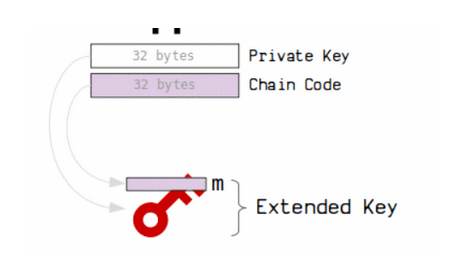
\includegraphics[width=0.7\textwidth]{images/extended_key.png}
    \caption[Example of the extended private key]{Example of the extended private key}
    \label{fig:extended_key}
\end{figure}

Driven by advances in both classical and quantum computing technologies, in May 2020, NIST recommended improving key length to 256 bits \cite{Barker2020}. It is unclear when scalable quantum computers will be available, and we will keep updating our system with the latest news on NIST publication.

Child key on the BIP32 key tree can only be derived from an extended key. From a security perspective, this is an excellent idea on how we can protect the child keys if the attackers get a hold of a stolen parent key. Because the extended key is collectively made up of a combination of key and chain code, attackers won’t have a better way to derive the children keys other than brute-forcing 32 bytes of extended entropy.

There are two types of extended keys. An extended private key is the combination of a private key and chain code and can be used to derive child private keys (and from them, child public keys) (see \autoref{fig:extended_key}). An extended public key is a public key and chain code, which can be used to create child public keys (public only). 

The index of the child key is a 32-bit integer, meaning that each extended key has $2^{32}$ child keys. This index number is divided into two ranges to easily determine between keys derived through the normal derivation function versus keys derived from hardened derivation. Index numbers between 0 and $2^{31}$–1 (0x0 to 0x7FFFFFFF) are used for normal derivation and the index numbers between $2^{31}$ and $2^{32}$–1 (0x80000000 to 0xFFFFFFFF) are used only for hardened derivation. Therefore, the normal child will have an index of less than $2^{31}$, whereas the hardened child index equals or is above  $2^{31}$.

We couldn’t find any reason behind why the author of BIP32 designed the parent extended keys to have $2^{32}$ total child keys each. Poulami Das et al. \cite{DBLP:conf/ccs/0003EFL021} investigated BIP32 with security analysis and experimented with a similar key derivation schema (BIP32-m) with only $2^{20}$ child keys, pointing out $2^{32}$ child keys won’t create any vulnerability on the system.

In the next part, we will represent an extended private key as (k, c), with k the normal private key, and c the chain code. An extended public key is represented as (K, c), with K = point(k) and c the chain code. The index is denoted to \textit{i}; to ease, $i_H$ is the index of a hardened key representing a number of i+$2^{31}$.

\bigskip
{\textbf{Convention}}

In the rest of this thesis, we will assume the public key cryptography used in Blockchain, namely elliptic curve cryptography using the field and curve parameters. Variables below are either:

\begin{itemize}
  \item Integers modulo the order of the curve (referred to as n).

  \item Coordinates of points on the curve.

  \item Byte sequences.
\end{itemize}

The addition (+) of two coordinate pairs is defined as the application of the EC group operation. Concatenation ($\parallel$) is the operation of appending one-byte sequence onto another.

As standard conversion functions, we assume:

\begin{itemize}
    \item $point(p)$: returns the coordinate pair resulting from EC point multiplication (repeated application of the EC group operation) of base point with the integer p.
  
    \item $ser_{32}(i)$: serialize a 32-bit unsigned integer $i$ as a 4-byte sequence, most significant byte first.
  
    \item $ser_{256}(p)$: serializes the integer $p$ as a 32-byte sequence, most significant byte first.
    \item $ser_P(P)$: serializes the coordinate pair $P = (x,y)$ as a byte sequence using the compressed form: $(0x02$ or $0x03) \parallel ser256(x)$, where the header byte depends on the parity of the omitted $y$ coordinate. 0x02 if $y$ is positive and 0x03 if $y$ is negative.
    \item $parse_{256}(p)$: interprets a 32-byte sequence as a 256-bit number, most significant byte first.
\end{itemize}


\bigskip
{\textbf{Master Extended Key generation function}}

Master extended key is the first key to be generated from the root seed. A master key also possesses a size of $2^{512}$ where 256 first bits is the master private key and the last 256 bits is the chain code. From the master private key, we can calculate the master public key.

Pseudo-code of generation function is as below:

\begin{itemize}
    \item Generate a seed byte sequence S of a chosen length (between 128 and 512 bits; 256 bits is advised) from a (pseudo) random number generator (PRNG).
    
    \begin{quote}
        The PRNG, as mentioned in Section \ref{chap:background}, is recommended to produce a root seed. However, BIP39 \cite{github/bip0039} invented a method to create a seed from mnemonic code or mnemonic sentence entropy. We will discuss BIP39 in Section \ref{SLIP10} . Ideally, the creation of BIP39 helps users to maintain their wallets more efficiently since secure random sentences (12 to 24 words) are more comfortable than protecting a random byte sequence.
    \end{quote}
    
    \item Calculate I = HMAC-SHA512(Key = "Bitcoin seed", Data = S)
    
        
    \begin{quote}
        The HMAC function returns 512 bits of data (which is totally unpredictable) from a key and data component. BIP32 added the key "Bitcoin seed" to the function, although it could be arbitrary when deriving the master node from the seed. This is considered necessary to ensure proper domain separation between different elliptic curves or different types of key hierarchy generation schemas.    
    \end{quote}

    \item Split I into two 32-byte sequences, $I_L$ and $I_R$.
        
    \begin{quote}
        The result of the HMAC function with the size 512 bits (64 bytes) will be split into 32 bits left  $I_L$ and 32 bits right $I_R$.
    \end{quote}
    \item Use $parse_{256}$($I_L$) as the master secret key, and $I_R$ as master chain code.

    \begin{quote}
        Return 32 bits left $I_L$ as the secret key and 32 bits right $I_R$ as the extended chain code.
    \end{quote}

\end{itemize}
In case $I_L$ is 0 or  n (private key  order n), the master key is invalid. 

\begin{figure}[ht!]
    \centering
    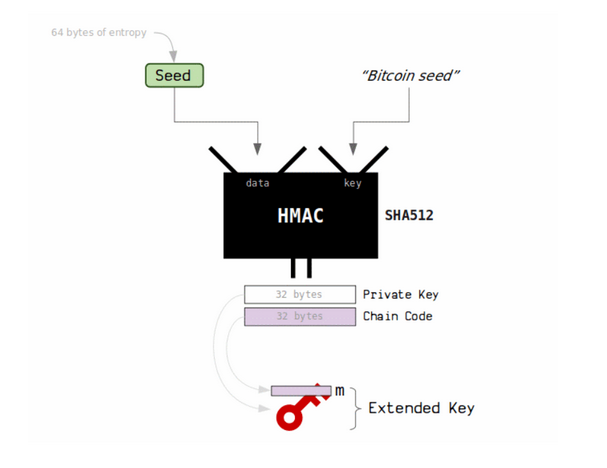
\includegraphics[width=0.7\textwidth]{images/masterbip32.png}
    \caption[Master Extended Key generation Process]{Master Extended Key generation Process}
    \label{fig:master_bip32}
\end{figure}

\subsubsection{SLIP10}
\label{SLIP10}

\subsubsection{BIP39}
\subsubsection{BIP44}

